\documentclass{article}
\usepackage[utf8]{inputenc}
\usepackage{geometry}
 \geometry{
 a4paper,
 total={170mm,257mm},
 left=20mm,
 top=20mm,
 }
 \usepackage{graphicx}
 \usepackage{titling}
 \usepackage{graphicx}
\usepackage{amsmath}
\usepackage{esint}
  
\DeclareMathOperator{\sech}{sech}
\DeclareMathOperator{\cosec}{cosec}
\DeclareMathOperator{\cosech}{cosech}

 \title{Assignment \textbf{1} (Lecture 1-5)
}
\author{Syed Suhaib Ahmad}
\date{\today}
 
 \usepackage{fancyhdr}
\fancypagestyle{plain}{%  the preset of fancyhdr 
    \fancyhf{} % clear all header and footer fields
    
    \fancyfoot[C]{1}
    \fancyhead[L]{8.02x - Electricity and Magnetism}
    \fancyhead[R]{\theauthor}
}
\makeatletter
\def\@maketitle{%
  \newpage
  \null
  \vskip 1em%
  \begin{center}%
  \let \footnote \thanks
    {\LARGE \@title \par}%
    \vskip 1em%
    %{\large \@date}%
  \end{center}%
  \par
  \vskip 1em}
\makeatother

\usepackage{lipsum}  
%\usepackage{cmbright}

\begin{document}

\maketitle


\subsubsection*{Problem 1.1 - Relative strengths of Gravitational and Electrostatic forces}
The gravitational force between two concentrated (“point-like") masses is very similar in its mathematical structure to the electrostatic force between two concentrated charges. The “strength" of these forces is, however, vastly different. To illustrate this, consider the following example. Somewhere in outer space are two identical dust grains, $50\,\mu$m in diameter, with mass density $2.5\,$g/cm$^3$. They are at a distance $d$ meters apart. If the grains were electrically neutral, free of other external forces, and have negligible relative velocity initially, they would eventually collide, gravitationally.
\\
\\Now suppose that both grains are electrically charged, each having $n$ “extra" electrons. Find the minimum value of $n$ that would prevent the gravitaional collision. Compare this with the approximate total number of electrons contained in one grain.
\\
\\\textbf{Solution}
\\
\\The mass of both grains is same since they both are identical. Their mass density, $\rho$, is $2.5\,\text{g/cm}^3$=$2.5\times10^3\,\text{kg/m}^3$. The mass of either of the grains is $m=\rho V=2.5\times10^3\,\text{kg/m}^3\times\frac{4}{3}\pi(25\times10^{-6})=1.6\times10^{-10}\,$kg. Using Newton's Law for gravitation, we can compute the gravitational force between the grains
\[F_g=\frac{GM_1M_2}{r^2}=\frac{Gm^2}{d^2}.\]
The total charge on each grain is given by $Q=-ne$ where $e$ is the elementary charge. To cancel out the effect of the gravitational force, the electric force between the grains should be equal to it.
\[F_g=F_e\Rightarrow\frac{Gm^2}{d^2}=\frac{n^2e^2}{4\pi\epsilon_0d^2}\Rightarrow n=\sqrt{\frac{4\pi\epsilon_0Gm^2}{e^2}}\approx0.09.\]
This value of $n$ shows that even a single extra electron on both grains ($n=1$) would prevent a collision due to their gravitational attraction. There are a total of $\frac{1.6\times10^{-10}}{1.67\times10^{-27}}\approx10^{17}$ nucleons on each of the grains. Assuming the grains are neutral, we can conclude that there is exactly one electron for every two nucleons (proton + neutron). Therefore, there are approximately $5\times10^{16}$ electrons in each grain.

\subsubsection*{Problem 1.2 - Electric field along the line passing through two point charges}
A point charge $Q_1=+3\,\mu C$ is placed at the origin, and a point charge $Q_2=-7\,\mu C$ is placed at $x=0.4$\,m on the $x-$axis of a cartesian coordinate system.
\begin{enumerate}
\item[(a)]Determine the electric field, $\Vec{\boldsymbol{E}}(x)=E(x)\boldsymbol{\hat{x}}$, at all points along the $x-$axis.
\item[(b)]At what point, if any, (apart from $|x|=\infty$), is $E(x)=0$?
\end{enumerate}
\textbf{Solution(a)}
\\
\\The electric field due to $Q_1$ alone is given by the expression: $\Vec{\boldsymbol{E_1}}=\frac{Q_1}{4\pi\epsilon_0r^2}\boldsymbol{\hat{r}}=\frac{Q_1}{4\pi\epsilon_0x^2}\boldsymbol{\hat{x}}$. Similarly the electric field due to $Q_2$, $\Vec{\boldsymbol{E_2}}$, is given by $\frac{Q_1}{4\pi\epsilon_0(x-0.4)^2}\boldsymbol{\hat{x}}$. The total electric field, $\Vec{\boldsymbol{E}}(x)$, is the sum of $\Vec{\boldsymbol{E_1}}$ and $\Vec{\boldsymbol{E_2}}$
\[\Vec{\boldsymbol{E}}(x)=\begin{cases}
    \frac{10^{-6}}{4\pi\epsilon_0}\left(\frac{3}{x^2}-\frac{7}{(x-0.4)^2}\right)\boldsymbol{\hat{x}}&-\infty<x<\infty
    \\\frac{10^{-6}}{4\pi\epsilon_0}\left(-\frac{3}{x^2}+\frac{7}{(x-0.4)^2}\right)\boldsymbol{\hat{x}}&-\infty<x<0
    \\\frac{10^{-6}}{4\pi\epsilon_0}\left(\frac{3}{x^2}+\frac{7}{(x-0.4)^2}\right)\boldsymbol{\hat{x}}&0<x<0.4
    \\\frac{10^{-6}}{4\pi\epsilon_0}\left(\frac{3}{x^2}-\frac{7}{(x-0.4)^2}\right)\boldsymbol{\hat{x}}&0.4<x<\infty\,\,.
\end{cases}\]
\textbf{Solution(b)}
\\
\\Upon plotting $\Vec{\boldsymbol{E}}(x)$ against $x$ for $x<0$, it can be seen that electric field is zero at $x=-0.758$\,m. Other than this value and $|x|=\infty$, there is no point at which $\Vec{\boldsymbol{E}}(x)$ is zero. In the interval $0<x<0.4$, $\Vec{\boldsymbol{E}}(x)$ is never zero as sum of two positive numbers is always greater than zero. Likewise, the negative charge, which is greater in magnitude, is always closer in the range $0.4<x<\infty$, thus electric field is always non-zero in this interval.

\subsubsection*{Problem 1.3 - Continuous charge distribution}
A thin rod bent into the shape of an arc of a circle of radius $R$ carries a uniform charge per unit length $\lambda$. The arc subtends a total angle $2\theta_0$, symmetric about the $x-$axis. Determine the electric field $\Vec{\boldsymbol{E}}$ at the origin $O$.
\begin{figure}[h]
        \centering
        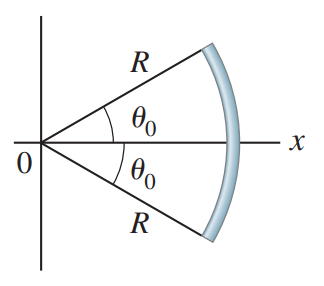
\includegraphics[width=0.25\linewidth]{figs/fig_prob_1.3.png}
       % \caption{Caption}
       % \label{fig:enter-label}
    \end{figure}
\\\textbf{Solution}
\\
\\Consider a small length element $dl$. The charge carried by this element is $dq=\lambda\,dl=\lambda\,Rd\theta$. The electric field due to this element is
\[d\Vec{\boldsymbol{E}}=\frac{\lambda\,Rd\theta}{4\pi\epsilon_0R^2}\boldsymbol{\hat{r}}=\frac{\lambda\,d\theta}{4\pi\epsilon_0R}(-\boldsymbol{\hat{i}}\cos\theta-\boldsymbol{\hat{j}}\sin\theta).\]
The electric field has only an $x-$component since
\[\int_{-\theta_0}^{\theta_0}\sin\theta\,d\theta=\left[-\cos\theta\right]_{-\theta_0}^{\theta_0}=-\cos\theta_0+\cos(-\theta_0)=0.\]
Integrating from $\theta=-\theta_0$ to $\theta=\theta_0$ gives the total electric field at the origin.
\[\Vec{\boldsymbol{E}}=-\boldsymbol{\hat{i}}\frac{\lambda}{4\pi\epsilon_0R}\int_{-\theta_0}^{\theta_0}\cos\theta\,d\theta=-\boldsymbol{\hat{i}}\frac{\lambda}{4\pi\epsilon_0R}\times2\sin\theta_0=-\boldsymbol{\hat{i}}\frac{\lambda\sin\theta_0}{2\pi\epsilon_0R}.\]

\subsubsection*{Problem 1.4 - E-field of a uniformly charged disk}
A disk of radius $R$ carries a uniform surface density $\sigma$. The $z-$axis passes through the center $O$. The total charge, $Q$, on the disk is thus $Q=\pi R^2\sigma$.
\begin{enumerate}
\item[(a)]What is the electric field $\Vec{\boldsymbol{E}}$ (magnitude and direction) at a point $P$ a distance $z$ above the center of the disk? Express your answer for $E_z$ in terms of $Q$, $R$, $\epsilon_0$ and $z$.
\item[(b)]Using the binomial expansion for $\sqrt{z^2+R^2}$, find simplified expressions for $E_z$ in two limiting cases:
\\(i) $z^2<<R^2$\,\,\,\,\,\,\,\,\,\,\,\,\,\,\,(ii) $z^2>>R^2$.
\item[(c)]Compare your result in case (ii) with the result you can obtain by making use of Coulomb's Law for a point-like charge.
\item[(d)]Using Gauss's Law (choose a proper “pillbox"), calculate $E_z$ near point $O$ for case (i); compare your answer with (c).
\end{enumerate}
\textbf{Solution(a)}
\\
\\Consider a ring of radius $r$ and width $dr$. The charge on this ring is $\sigma(2\pi\,rdr)$. By taking symmetry into account, it can be seen that the electric field at point P is in the positive $z-$direction. Thus, the electric field due to this ring is given by
\[d\Vec{\boldsymbol{E}}=\frac{\sigma(2\pi\,rdr)}{4\pi\epsilon_0s^2}\boldsymbol{\hat{r}}=\frac{\frac{Q}{\pi\,R^2}\times2\pi\,rdr}{4\pi\epsilon_0\left(r^2+z^2\right)}\boldsymbol{\hat{k}}\cos\theta=\frac{Qzrdr}{2\pi\epsilon_0R^2\left(r^2+z^2\right)^{\frac{3}{2}}}\boldsymbol{\hat{k}}\]
Integrating over the entire radius of disk gives
\[\Vec{\boldsymbol{E}}=\boldsymbol{\hat{k}}\frac{Qz}{2\pi\epsilon_0R^2}\int_{0}^{R}\frac{r}{\left(r^2+z^2\right)^{\frac{3}{2}}}\,dr=\boldsymbol{\hat{k}}\frac{Qz}{2\pi\epsilon_0R^2}\int_{0}^{R}\frac{d}{dr}\left(-\left(r^2+z^2\right)^{-\frac{1}{2}}\right)\,dr\]
\[=\boldsymbol{\hat{k}}\frac{Qz}{2\pi\epsilon_0R^2}\left[-\frac{1}{\sqrt{r^2+z^2}}\right]_{0}^{R}=\boldsymbol{\hat{k}}\frac{Q}{2\pi\epsilon_0R^2}\left[1-\frac{z}{\sqrt{R^2+z^2}}\right].\]
\\
\\\textbf{Solution(b)}
\\
\\For case (i), the electric field, $\Vec{\boldsymbol{E}}$, can be written as $\boldsymbol{\hat{k}}\frac{Q}{2\pi\epsilon_0R^2}\left[1-\frac{z/R}{\sqrt{1+(z/R)^2}}\right]$ where $1-\frac{z^2}{2R^2}$ is a good approximation for $\left(1+(z/R)^2\right)^{-\frac{1}{2}}$. Hence,
\[E_z\approx\frac{Q}{2\pi\epsilon_0R^2}\left[1-\frac{z}{R}\left(1-\frac{z^2}{2R^2}\right)\right]\approx\frac{Q}{2\pi\epsilon_0R^2}.\]
Using the same approach, for case (ii), we first write the electric field as $\boldsymbol{\hat{k}}\frac{Q}{2\pi\epsilon_0R^2}\left[1-\frac{1}{\sqrt{1+(R/z)^2}}\right]$ where the term $\left(1+(R/z)^2\right)^{-\frac{1}{2}}$ can be approximated to $1-\frac{R^2}{2z^2}$. Therefore, the electric field now becomes:
\[E_z\approx\frac{Q}{2\pi\epsilon_0R^2}\left[1-\left(1-\frac{R^2}{2z^2}\right)\right]\approx\frac{Q}{4\pi\epsilon_0z^2}.\]
\textbf{Solution(c)}
\\
\\The expression obtained in case (ii) is same as Coulomb's Law for a point-like charge as $E_z\propto\frac{1}{z^2}$. (The entire disk is considered as a point-like charge and $z$ is the distance between point $P$ and disk.)
\\
\\\textbf{Solution(d)}
\\
\\When $z<<R$, the disk resembles an infinite plane of uniform charge density $\sigma$. Thus, a Gaussian surface in the shape of a cylinder is suitable in this planar symmetry. This Gaussian "pillbox" has three surfaces; top ($S_1$), bottom ($S_2$), and a curved surface ($S_3$). Since the electric field is perpendicular to $S_3$, electric flux is zero through this curved surface. Both $S_1$ and $S_2$ have equal areas ($A_1=A_2=A$) and are under constant electric field ($E_1=E_2=E_z$). Therefore, the total electric flux through the pillbox is 
\[\Phi_E=\oiint_{S}\Vec{\boldsymbol{E}}\cdot d\Vec{\boldsymbol{A}}=\iint_{S_1}\Vec{\boldsymbol{E}}_1\cdot d\Vec{\boldsymbol{A}}_1+\iint_{S_2}\Vec{\boldsymbol{E}}_2\cdot d\Vec{\boldsymbol{A}}_2+\iint_{S_3}\Vec{\boldsymbol{E}}_3\cdot d\Vec{\boldsymbol{A}}_3\]
\[=E_1A_1+E_2A_2+0=EA+EA=2E_zA.\]
The enclosed charge is $Q_{\text{enc}}=\sigma A\Rightarrow\frac{QA}{\pi R^2}$. Applying Gauss's Law to the pillbox
\[2E_zA=\frac{Q_{\text{enc}}}{\epsilon_0}=\frac{QA}{\pi\epsilon_0R^2}\Rightarrow E_z=\frac{Q}{2\pi\epsilon_0R^2}.\]
This result is exactly the same as the expression obtained in b(i).

\subsubsection*{Problem 1.5 - Electric dipole}
Show that at points along the axis of a dipole (along the same line that contains $+Q$ and $-Q$), the electric
field has magnitude $E=\frac{1}{4\pi\epsilon_0}\frac{2p}{r^3}$ for $r>>l$, where $r$ is the distance from a point to the center of the dipole and $l$ is the distance between the two charges.
In what direction does $\Vec{\boldsymbol{E}}$ point? 
\\
\\\textbf{Solution}
\\
\\For this problem, we assume that the charges are placed on $x-$axis with both charges located at a distance of $l/2$ from the origin. Electric field due to the individual charges at point $A$ located at a distance $r$ along the $x-$axis ($r>0$) is given by
\[\Vec{\boldsymbol{E}}_{+Q}=\frac{+Q}{4\pi\epsilon_0(r-l/2)^2}\boldsymbol{\hat{x}}\,\,\,\,\,\,\text{and}\,\,\,\,\,\,\Vec{\boldsymbol{E}}_{-Q}=\frac{-Q}{4\pi\epsilon_0(r+l/2)^2}\boldsymbol{\hat{x}}.\]
To find the net electric field at $A$, we vectorially add the individual electric fields of the charges.
\[\Vec{\boldsymbol{E}}=\frac{+Q}{4\pi\epsilon_0(r-l/2)^2}\boldsymbol{\hat{x}}+\frac{-Q}{4\pi\epsilon_0(r+l/2)^2}\boldsymbol{\hat{x}}=\frac{Q}{4\pi\epsilon_0r^2}\left[\frac{1}{(1-l/2r)^2}-\frac{1}{(1+l/2r)^2}\right]\boldsymbol{\hat{x}}.\]
As already mentioned in the statement of the problem, $r$ is much greater than $l$, thus the binomial expansion can be used here. $(1-l/2r)^{-2}$ can be approximated to $1+l/r$ and similarly $(1+l/2r)^{-2}$ can be written as $1-l/r$ for $l/2r<<1$. Substituting these results into the equation for the net electric field gives
\[\Vec{\boldsymbol{E}}=\frac{Q}{4\pi\epsilon_0r^2}\left[1+l/r-1+l/r\right]\boldsymbol{\hat{x}}=\frac{2Ql}{4\pi\epsilon_0r^3}\boldsymbol{\hat{x}}\Rightarrow|\Vec{\boldsymbol{E}}|=\frac{2p}{4\pi\epsilon_0r^3}.\]
The electric field points in the positive $x-$direction as the positive charge $+Q$ is always closer to $A$.

\subsubsection*{Problem 1.6 - Gauss's law and the Superposition Principle}
We have and infinite, non-conducting, sheet of negligible thickness carrying a negative uniform surface charge density $\sigma$ and, next to it, an infinite parallel slab of thickness $D$ with positive uniform volume charge density $\rho$. All charges are fixed. Calculate the direction and magnitude of the electric field.
 \begin{figure}[h]
        \centering
        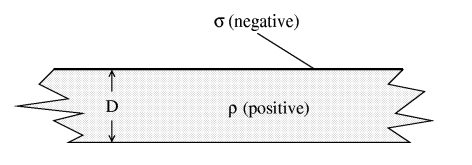
\includegraphics[width=0.5\linewidth]{figs/fig_prob_1.6.png}
       % \caption{Caption}
       % \label{fig:enter-label}
    \end{figure}
\begin{enumerate}
    \item[(a)]Above the negatively charged sheet.
    \item[(b)]Below the slab.
    \item[(c)]In the slab.
\end{enumerate}
\textbf{Solution(a)}
\\
\\Consider a coordinate system with the $z-$axis perpendicular to the sheet and slab and $z=0$ at the middle of the slab. We define three regions;
\[R_1: z>\frac{D}{2},\,\,\,\,\,\,\,\,\,\,R_2:|z|<\frac{D}{2},\,\,\,\,\,\,\,\,\,\,R_3:z<-\frac{D}{2}.\]
Part (a) asks us to find the the net electric field in the region $R_1$. We first find the electric field due to sheet and slab and then sum them vectorially to find their resultant. In all three cases, Gauss's Law can be used as both sheet and slab posses planar symmetry. 
\[\oiint\Vec{\boldsymbol{E}}_{\text{sheet}}\cdot d\Vec{\boldsymbol{A}}=\frac{\sigma A}{\epsilon_0}\Rightarrow2E_{\text{sheet}}A=\frac{\sigma A}{\epsilon_0}\Rightarrow\Vec{\boldsymbol{E}}_{\text{sheet}}=\frac{\sigma}{2\epsilon_0}\boldsymbol{\hat{z}}\]
\[\oiint\Vec{\boldsymbol{E}}_{\text{slab}}\cdot d\Vec{\boldsymbol{A}}=\frac{\rho AD}{\epsilon_0}\Rightarrow2E_{\text{slab}}A=\frac{\rho AD}{\epsilon_0}\Rightarrow\Vec{\boldsymbol{E}}_{\text{slab}}=\frac{\rho D}{2\epsilon_0}\boldsymbol{\hat{z}}.\]
\[\Vec{\boldsymbol{E}}_{\text{net}_1}=\Vec{\boldsymbol{E}}_{\text{sheet}}+\Vec{\boldsymbol{E}}_{\text{slab}}=\frac{\sigma}{2\epsilon_0}\boldsymbol{\hat{z}}+\frac{\rho D}{2\epsilon_0}\boldsymbol{\hat{z}}=\frac{(\sigma+\rho D)}{2\epsilon_0}\boldsymbol{\hat{z}}.\]
\textbf{Solution(b)}
\\
\\The electric field in $R_3$ is the same as in $R_1$ but in the opposite direction. Hence, $\Vec{\boldsymbol{E}}_{\text{net}_2}=-\frac{(\sigma+\rho D)}{2\epsilon_0}\boldsymbol{\hat{z}}.$
\\
\\\textbf{Solution(c)}
\\
\\For $R_3$ we choose the same Gaussian surface but this time its length is $2z$ where $z<\frac{D}{2}$. The electric field due to the sheet is same as it was in part(a) but in opposite direction as $R_3$ is below the negatively charged sheet.
\[\Vec{\boldsymbol{E}}_{\text{sheet}}=-\frac{\sigma}{2\epsilon_0}\boldsymbol{\hat{z}}\]
\[\oiint\Vec{\boldsymbol{E}}_{\text{slab}}\cdot d\Vec{\boldsymbol{A}}=\frac{2\rho Az}{\epsilon_0}\Rightarrow2E_{\text{slab}}A=\frac{2\rho Az}{\epsilon_0}\Rightarrow\Vec{\boldsymbol{E}}_{\text{slab}}=\frac{\rho z}{\epsilon_0}\boldsymbol{\hat{z}}.\]
\[\Vec{\boldsymbol{E}}_{\text{net}_3}=-\frac{\sigma}{2\epsilon_0}\boldsymbol{\hat{z}}+\frac{\rho z}{\epsilon_0}\boldsymbol{\hat{z}}=\left(\frac{\rho z}{\epsilon_0}-\frac{\sigma}{2\epsilon_0}\right)\boldsymbol{\hat{z}}.\]

\subsubsection*{Problem 1.7 - Two spherical charged shells}
Two thin concentric spherical shells of radii $r_1$ and $r_2$ ($r_1<r_2$) contain uniform surface charge densities $\sigma_1$ and $\sigma_2$ respectively. Determine the electric field for
\begin{enumerate}
    \item[(a)]$0<r<r_1$
    \item[(b)]$r_1<r<r_2$
    \item[(c)]$r>r_2$.
    \item[(d)]Under what conditions will $E=0$ for $r>r_2$?
    \item[(e)]Under what conditions will $E=0$ for $r_1<r<r_2$? 
\end{enumerate}
\textbf{Solution(a)}
\\
\\For simplicity, we choose a Gaussian surface in the shape of a spherical shell with radius $r$. Now for $0<r<r_1$, the electric field is zero as no charge is enclosed by the Gaussian surface.
\\
\\\textbf{Solution(b)}
\\
\\From symmetry arguments we see that electric field is in radial direction. The enclosed charge is $\sigma_1(4\pi r_1^2)$.
\[E\times4\pi r^2=\frac{\sigma_1(4\pi r_1^2)}{\epsilon_0}\Rightarrow E=\left(\frac{r_1}{r}\right)^2\frac{\sigma_1}{\epsilon_0}.\]
\textbf{Solution(c)}
\\
\\This time the total charge enclosed by the Gaussian surface is $Q=\sigma_1(4\pi r_1^2)+\sigma_2(4\pi r_2^2)$.
\[E\times4\pi r^2=\frac{\sigma_1(4\pi r_1^2)+\sigma_2(4\pi r_2^2)}{\epsilon_0}\Rightarrow E=\frac{\sigma_1 r_1^2+\sigma_2 r_2^2}{\epsilon_0r^2}.\]
\textbf{Solution(d)}
\\
\\The electric field can only be zero in this interval if $\sigma_1 r_1^2=-\sigma_2 r_2^2$, meaning that the two shells have same but opposite charges.
\\
\\\textbf{Solution(e)}
\\
\\For this scenario, $\sigma_1$ should be zero so there is no charge inside the Gaussian surface of radius $r_1<r<r_2$.

\subsubsection*{Problem 1.8 - Two concentric charged cylinders}
A thin cylindrical shell of radius $R_1$ is surrounded by a
second concentric cylindrical shell of radius $R_2$.
The inner shell has a total charge $+Q$ and the outer 
shell $-Q$. Assuming the length $l$ of the shells is much greater
than $R_1$ or $R_2$, determine the electric field as a function of $R$ (the perpendicular distance from the common axis of the cylinders) for 
\begin{enumerate}
    \item[(a)]$0<R<R_1$
    \item[(b)]$R_1<R<R_2$
    \item[(c)]$R>R_2$
    \item[(d)]What is the kinetic energy of an electron if it moves between (and concentric with) the shells in a circular orbit of radius $(R_1+R_2)/2$?
\end{enumerate}
\textbf{Solution(a)}
\\
\\Electric field is zero in this interval as $Q_{\text{enc}}=0$.
\\
\\\textbf{Solution(b)}
\\We choose a Gaussian surface in the form of a cylinder of radius $R$ and length $l$. The enclosed charge in this interval is $\frac{lQ}{L}$.
\[E\times2\pi Rl=\frac{lQ}{L\epsilon_0}\Rightarrow E=\frac{Q}{2\pi\epsilon_0LR}.\]
\textbf{Solution(c)}
\\
\\Again the electric field is zero as $Q_{\text{enc}}=\frac{lQ}{L}+\frac{-lQ}{L}=0$.
\\
\\\textbf{Solution(d)}
\\
\\The electric force on the electron is given by
\[F=eE=\frac{eQ}{\pi\epsilon_0L(R_1+R_2)}.\]
This electric force is equal to the the centripetal force of the electron so it maintains its motion.
\[\frac{eQ}{\pi\epsilon_0L(R_1+R_2)}=\frac{2m_ev^2}{(R_1+R_2)}\Rightarrow v=\sqrt{\frac{eQ}{2m_e\pi\epsilon_0L}}\]
Finally, we substitute this value of $v$ into the equation for kinetic energy.
\[K.E=\frac{1}{2}mv^2=\frac{1}{2}m_e\times\frac{eQ}{2m_e\pi\epsilon_0L}=\frac{eQ}{4\pi\epsilon_0L}.\]

\end{document}
